\begin{figure}
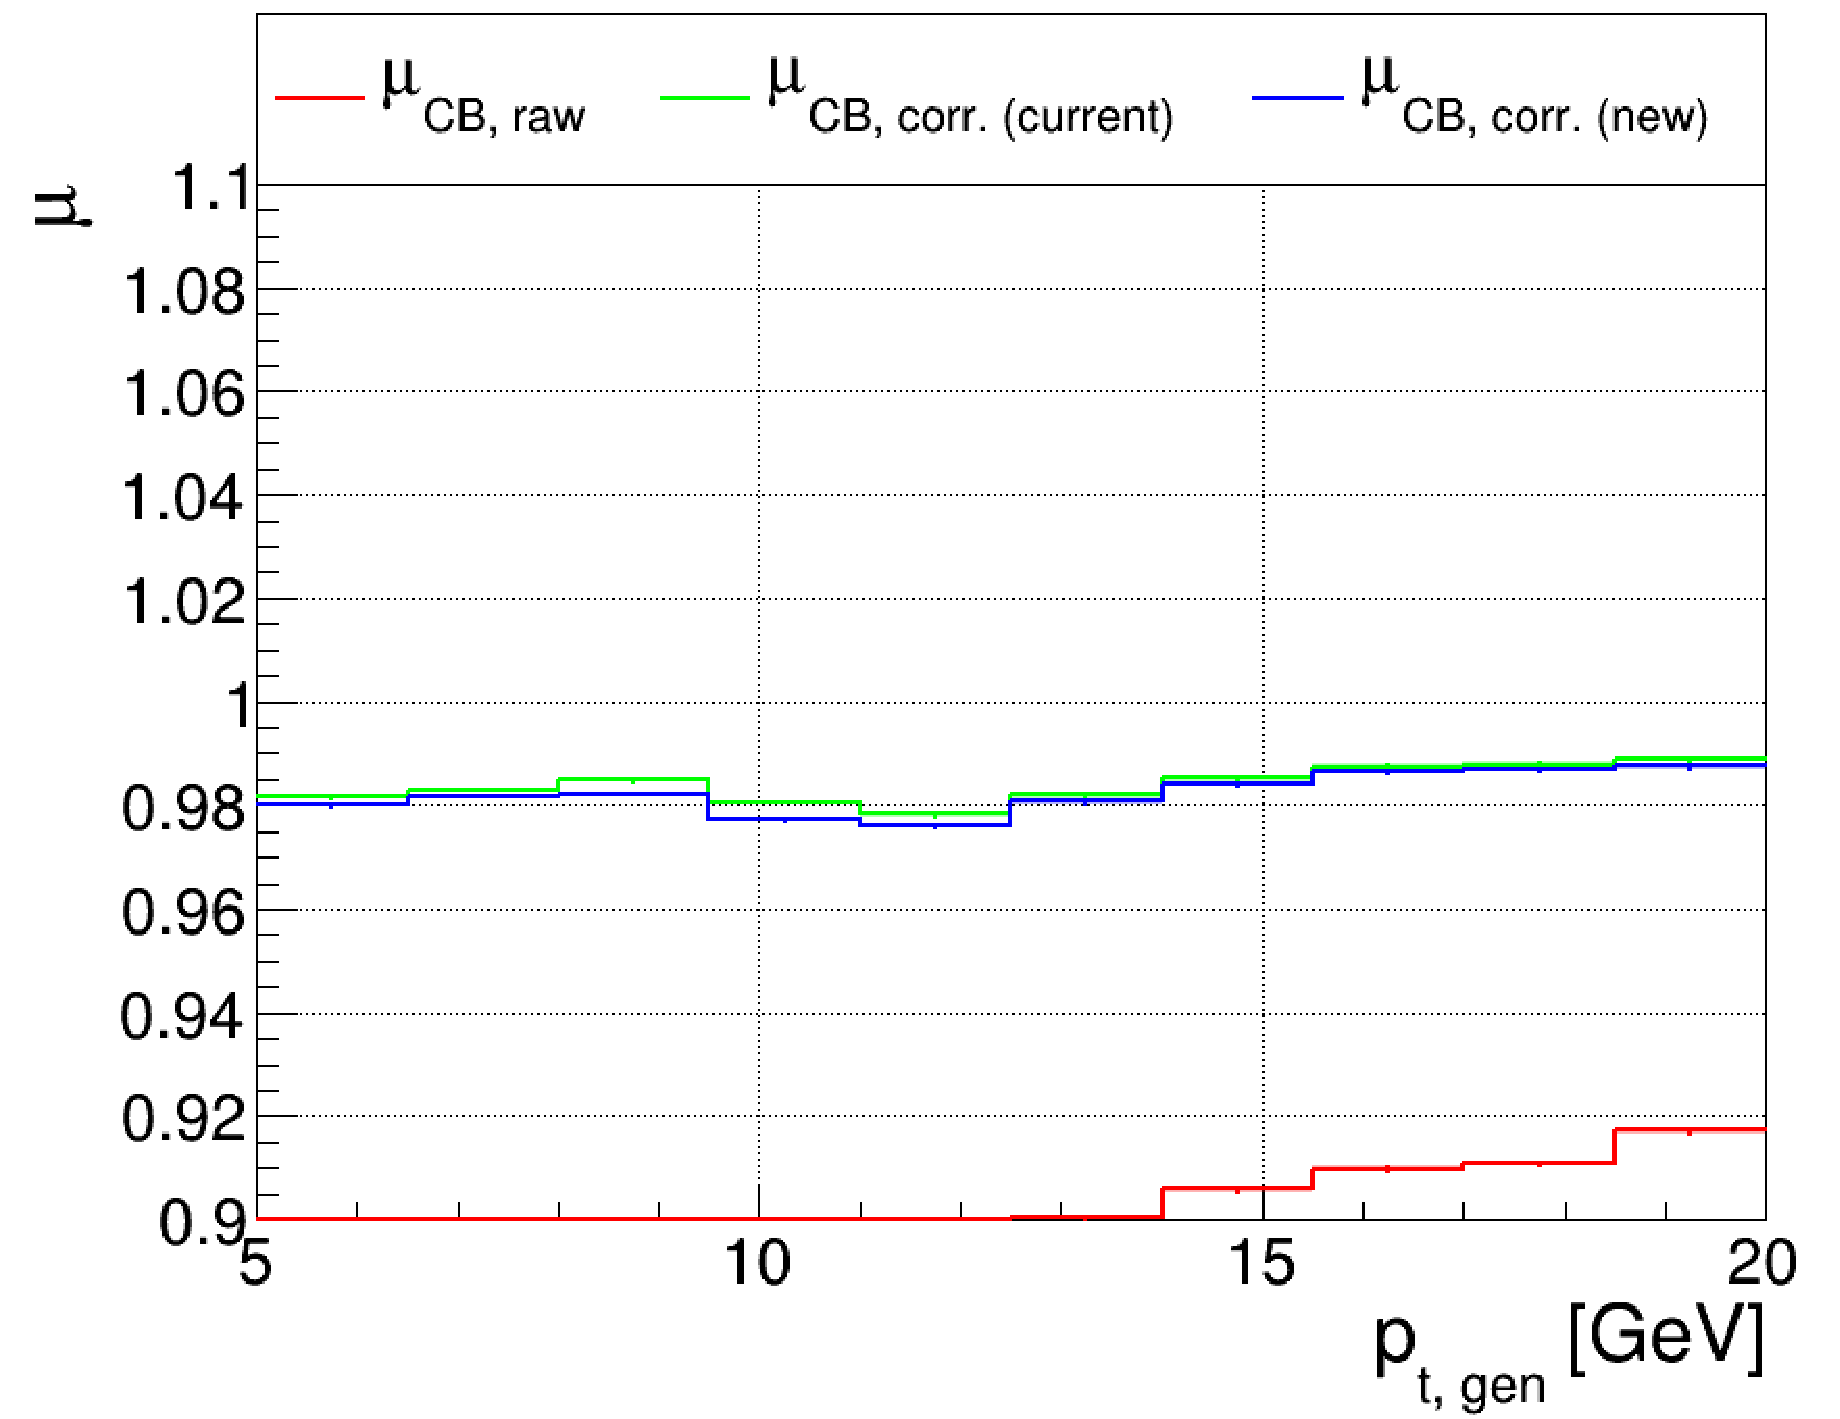
\includegraphics[width=0.495\textwidth]{./plots_pdf/ECAL_plots/plotsPU/EB/FULL/pdf/GENPT/EBFULL_GENPT_0005_0020_MuOverBins.pdf}
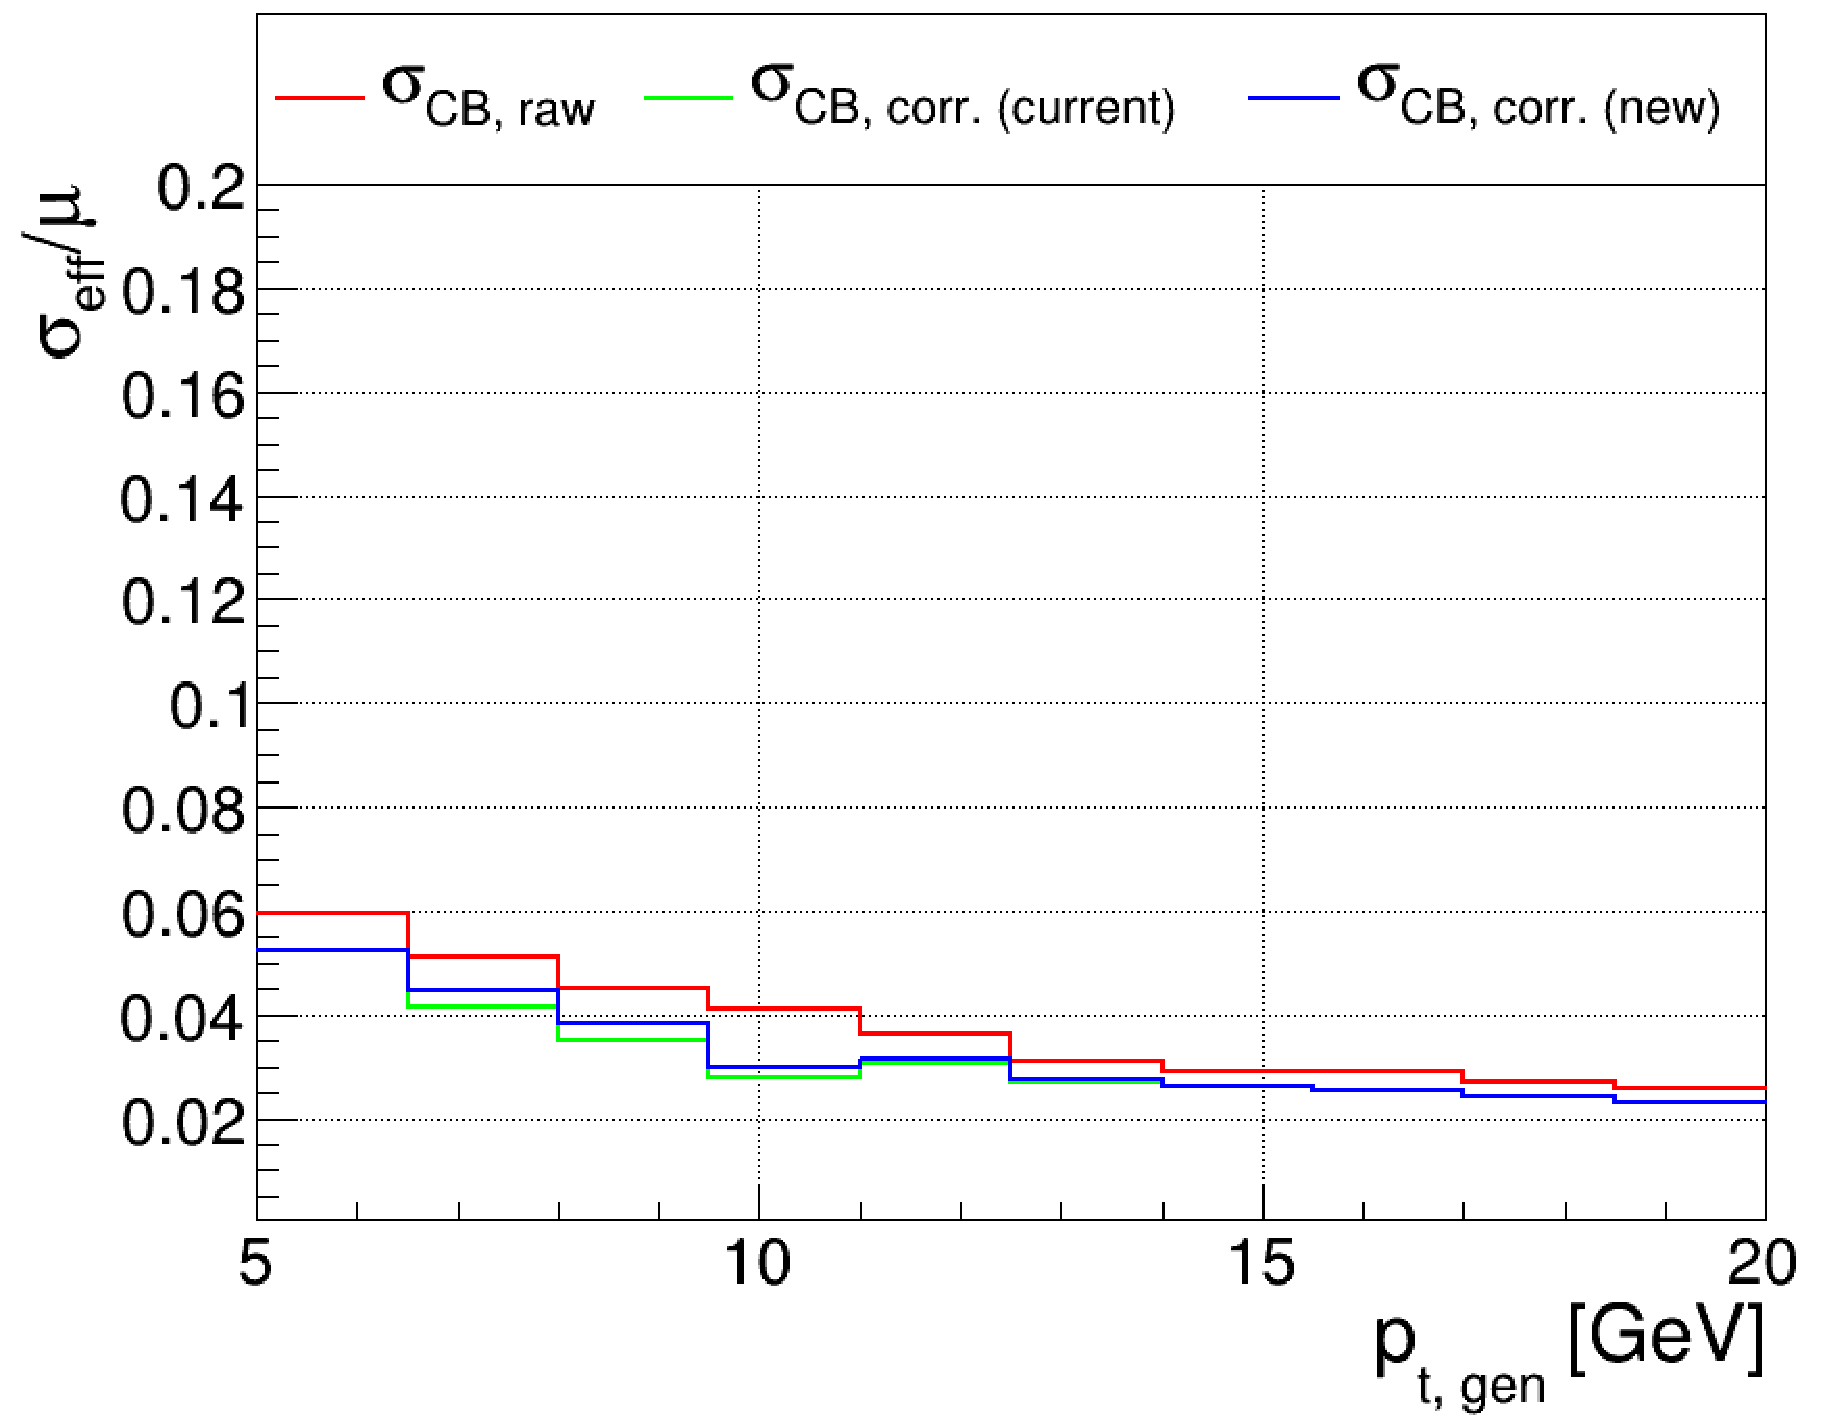
\includegraphics[width=0.495\textwidth]{./plots_pdf/ECAL_plots/plotsPU/EB/FULL/pdf/GENPT/EBFULL_GENPT_0005_0020_EffSigmaOverBins.pdf}

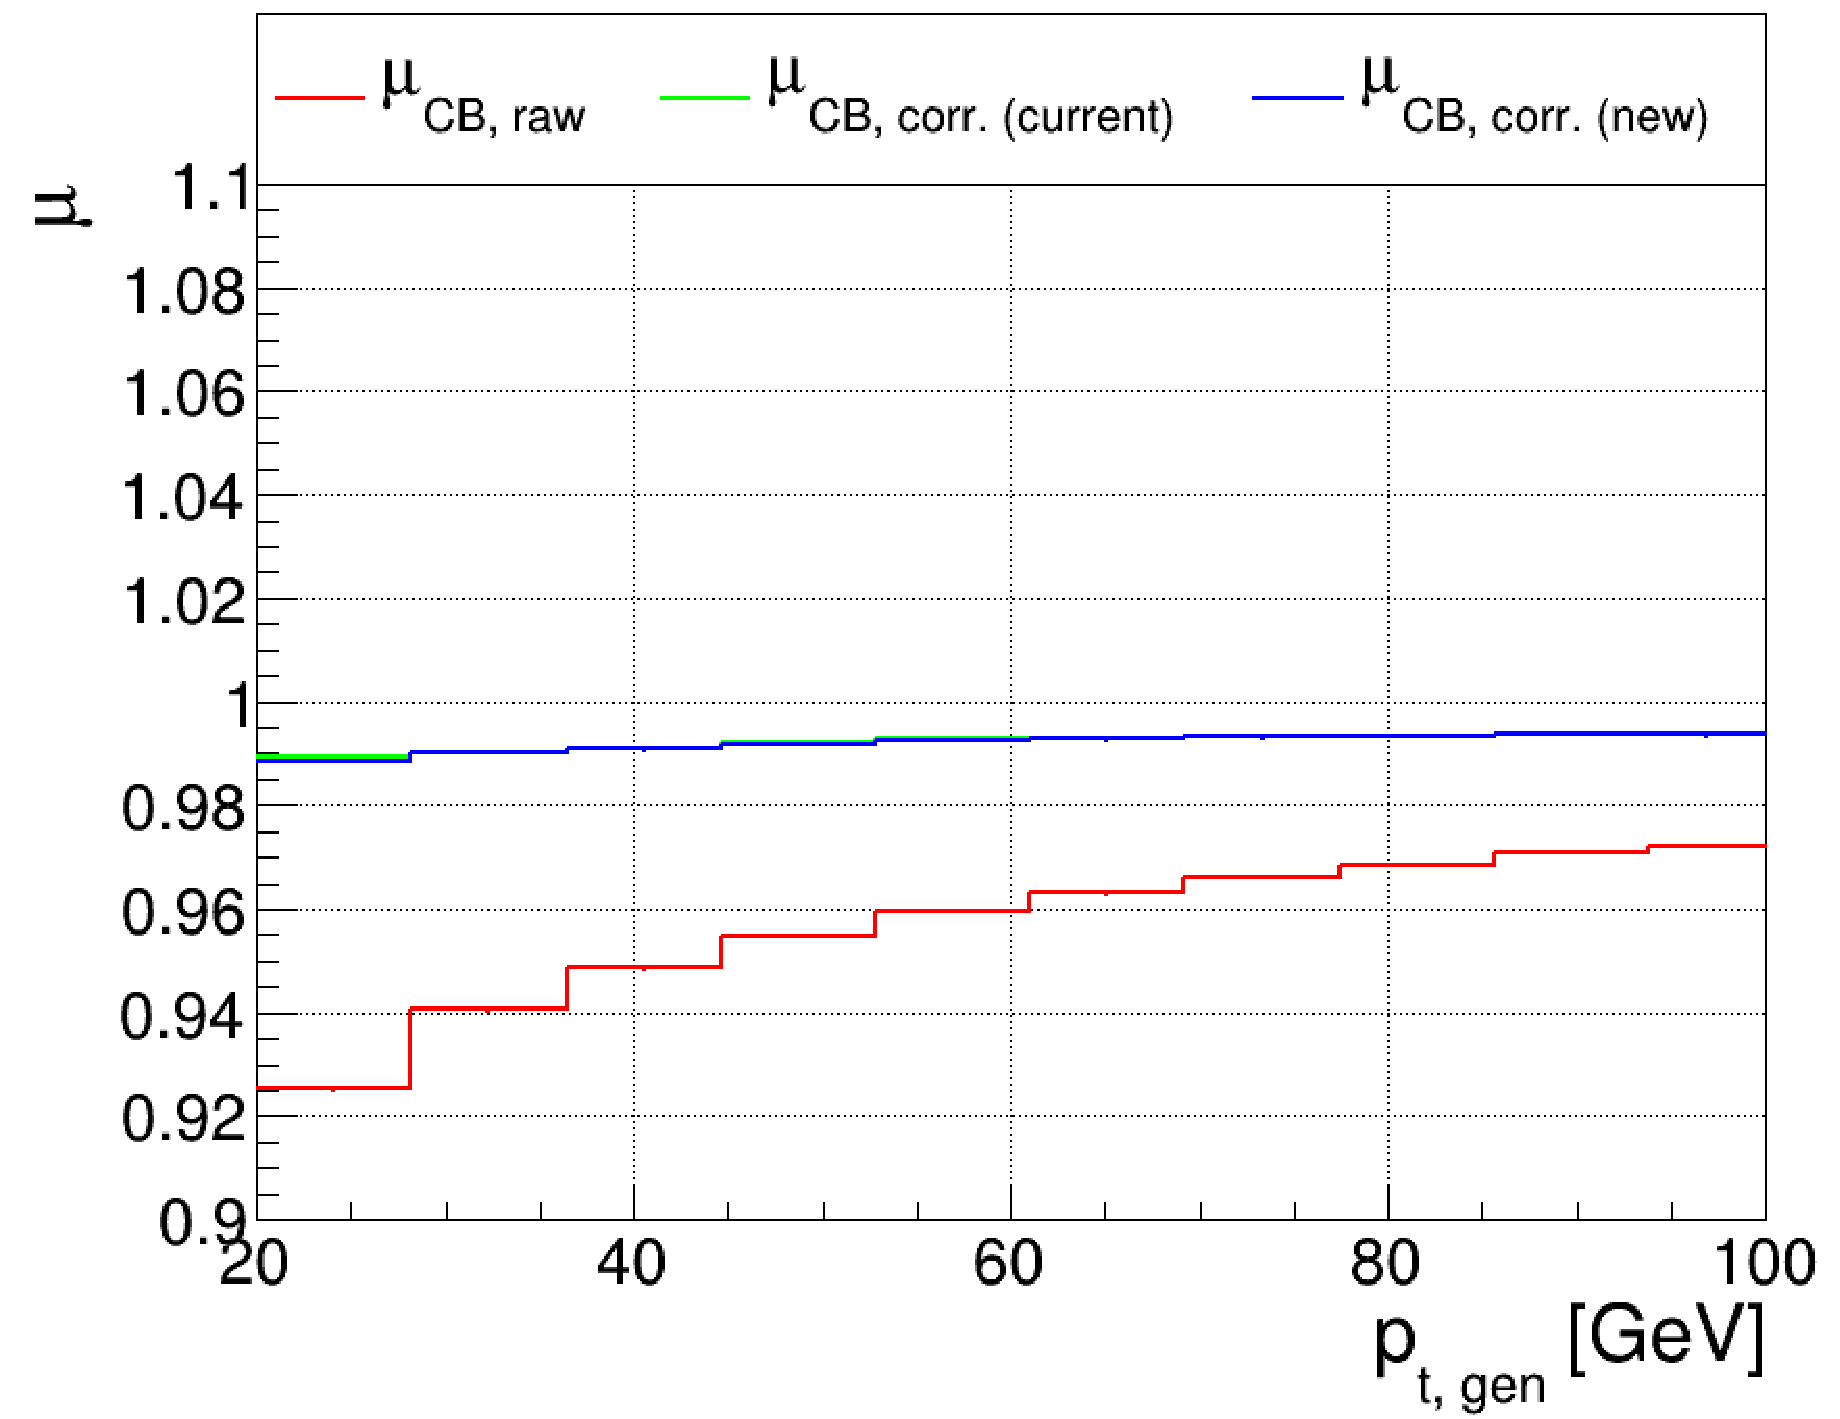
\includegraphics[width=0.495\textwidth]{./plots_pdf/ECAL_plots/plotsPU/EB/FULL/pdf/GENPT/EBFULL_GENPT_0020_0100_MuOverBins.pdf}
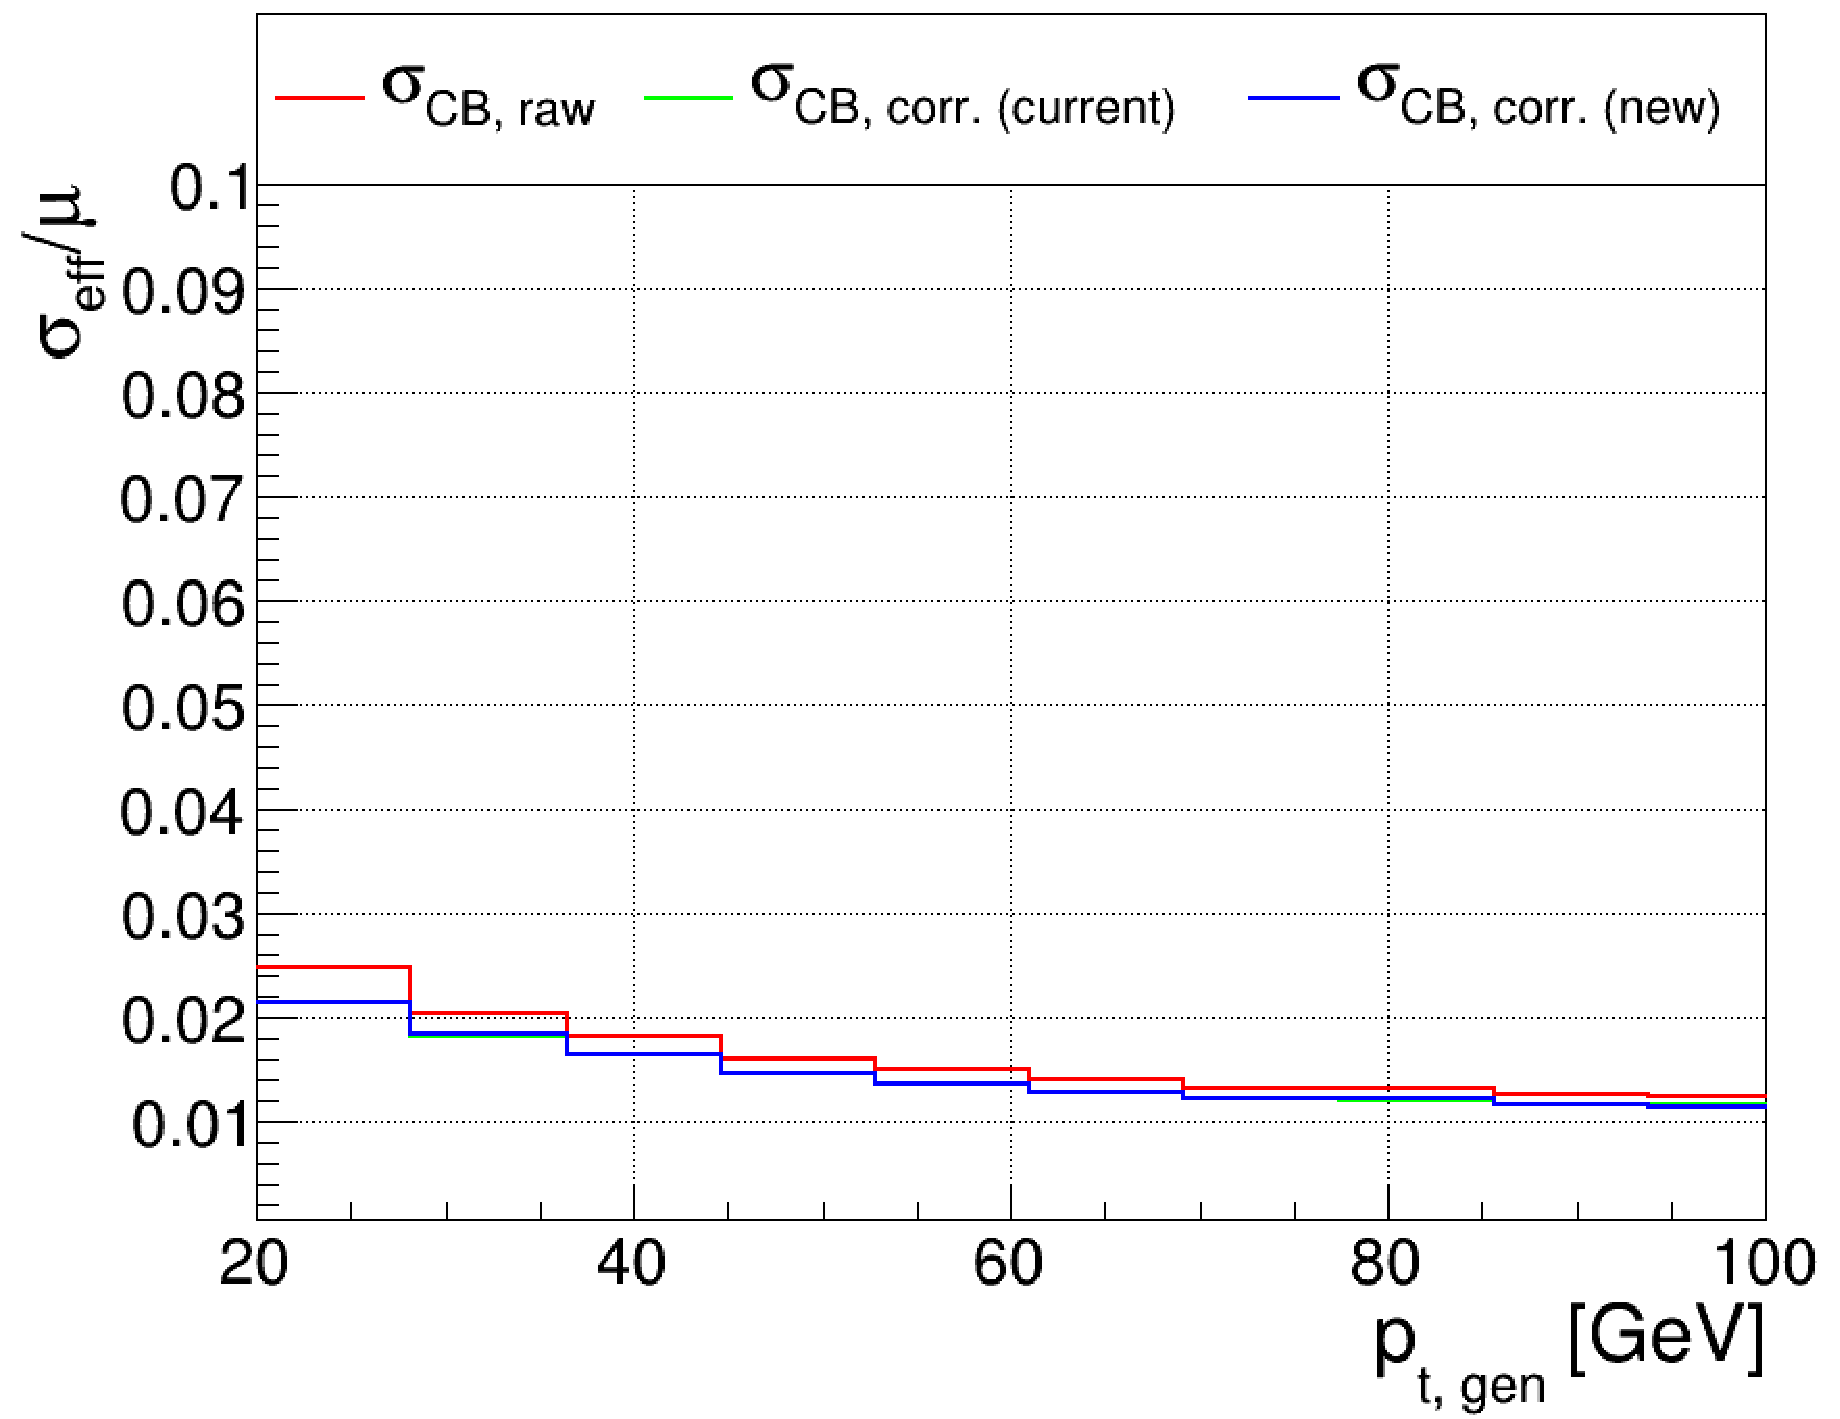
\includegraphics[width=0.495\textwidth]{./plots_pdf/ECAL_plots/plotsPU/EB/FULL/pdf/GENPT/EBFULL_GENPT_0020_0100_EffSigmaOverBins.pdf}

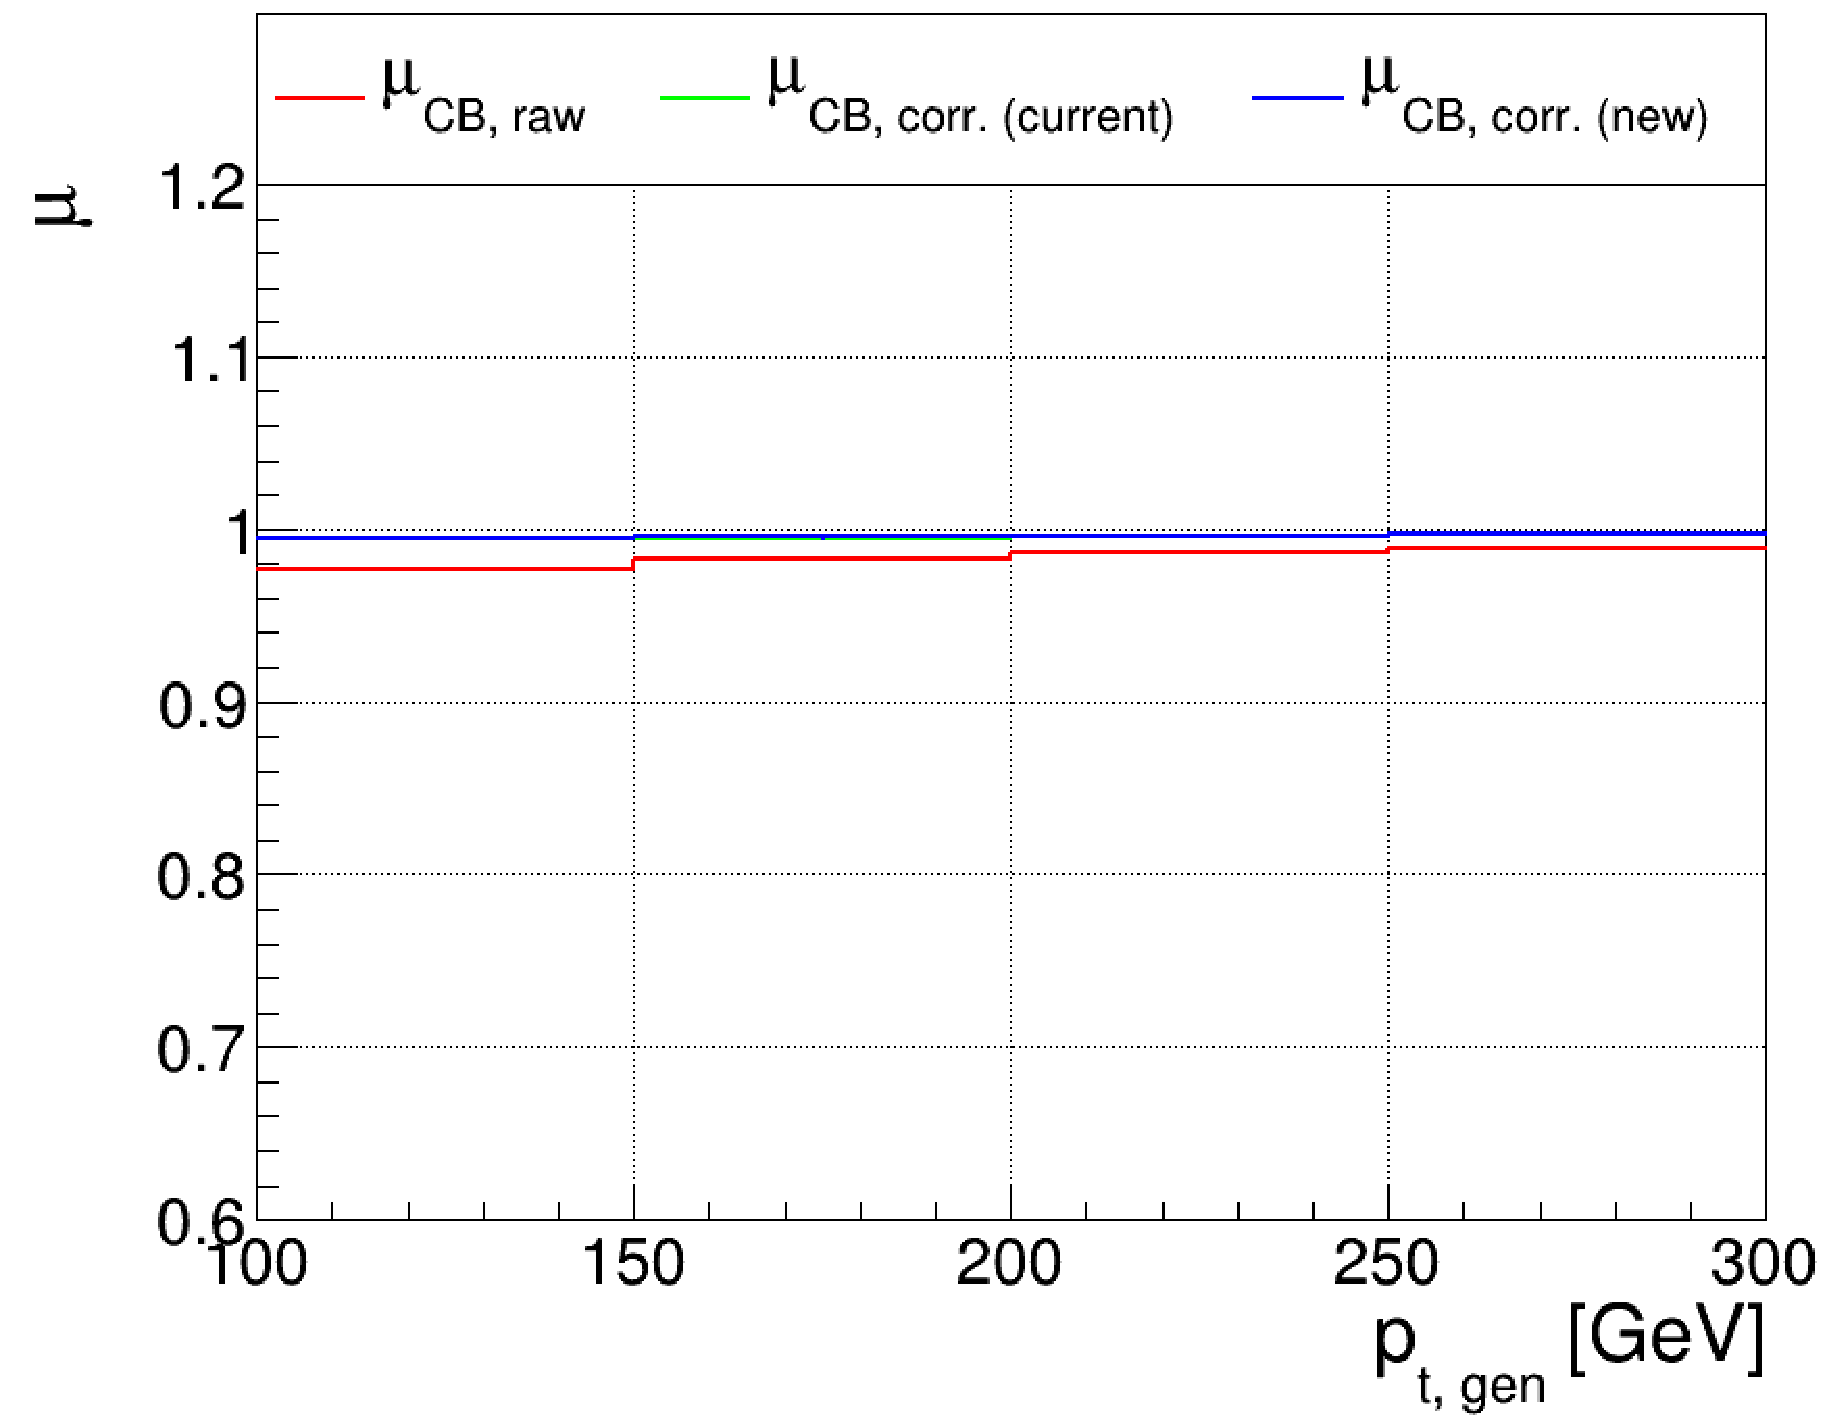
\includegraphics[width=0.495\textwidth]{./plots_pdf/ECAL_plots/plotsPU/EB/FULL/pdf/GENPT/EBFULL_GENPT_0100_0300_MuOverBins.pdf}
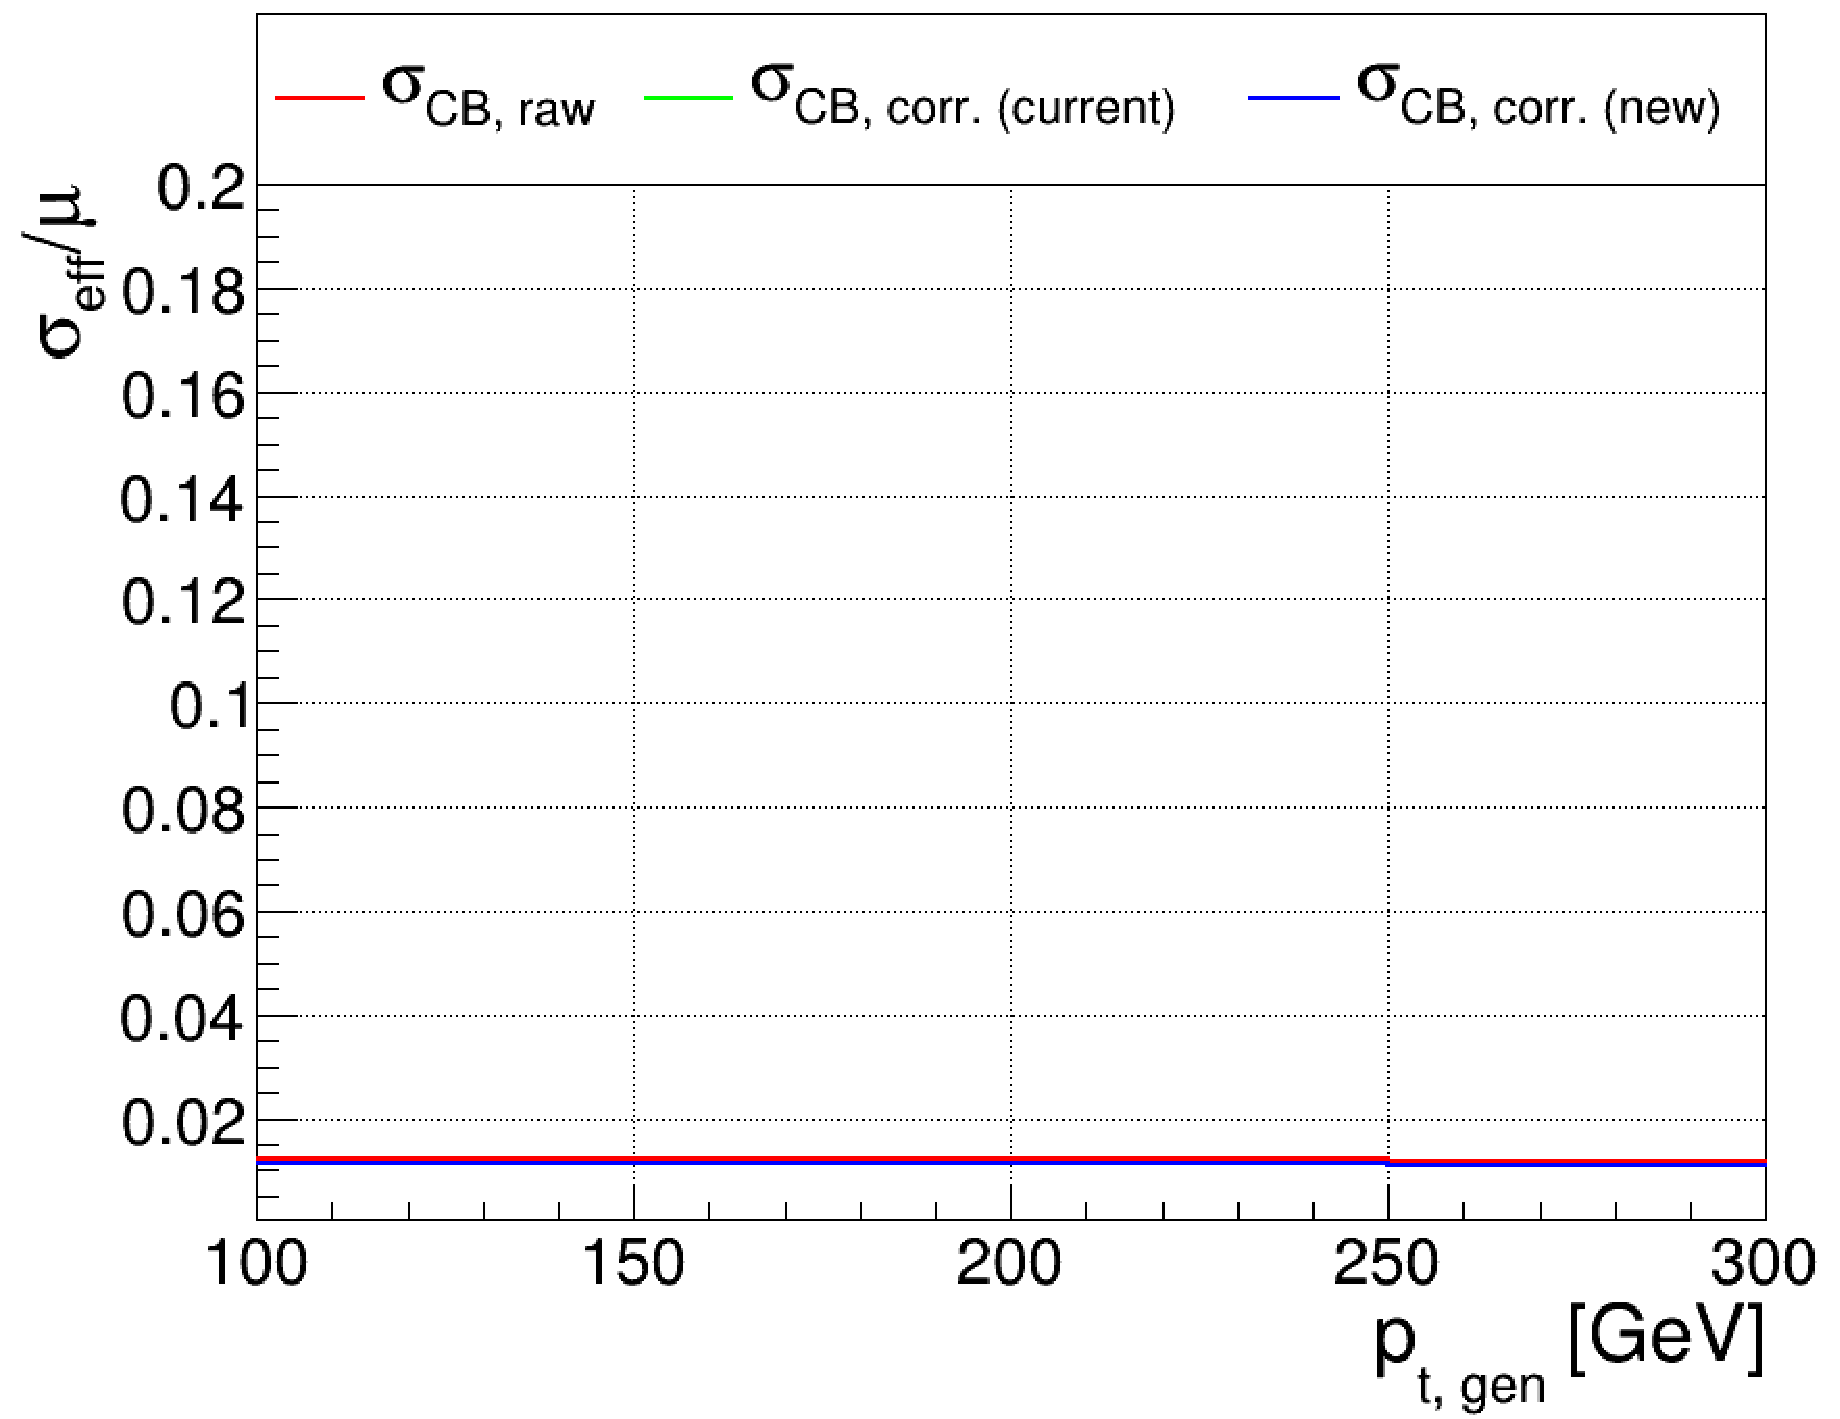
\includegraphics[width=0.495\textwidth]{./plots_pdf/ECAL_plots/plotsPU/EB/FULL/pdf/GENPT/EBFULL_GENPT_0100_0300_EffSigmaOverBins.pdf}

\caption [Energy response of PF ECAL cluster vs \pt for PU EB Full readout senario]{PU EB Full Readout (top) low \pt, (middle) mid \pt, (bottom) high \pt}
\label{fig:PU_EBFULL_pt}
\end{figure}


\begin{figure}
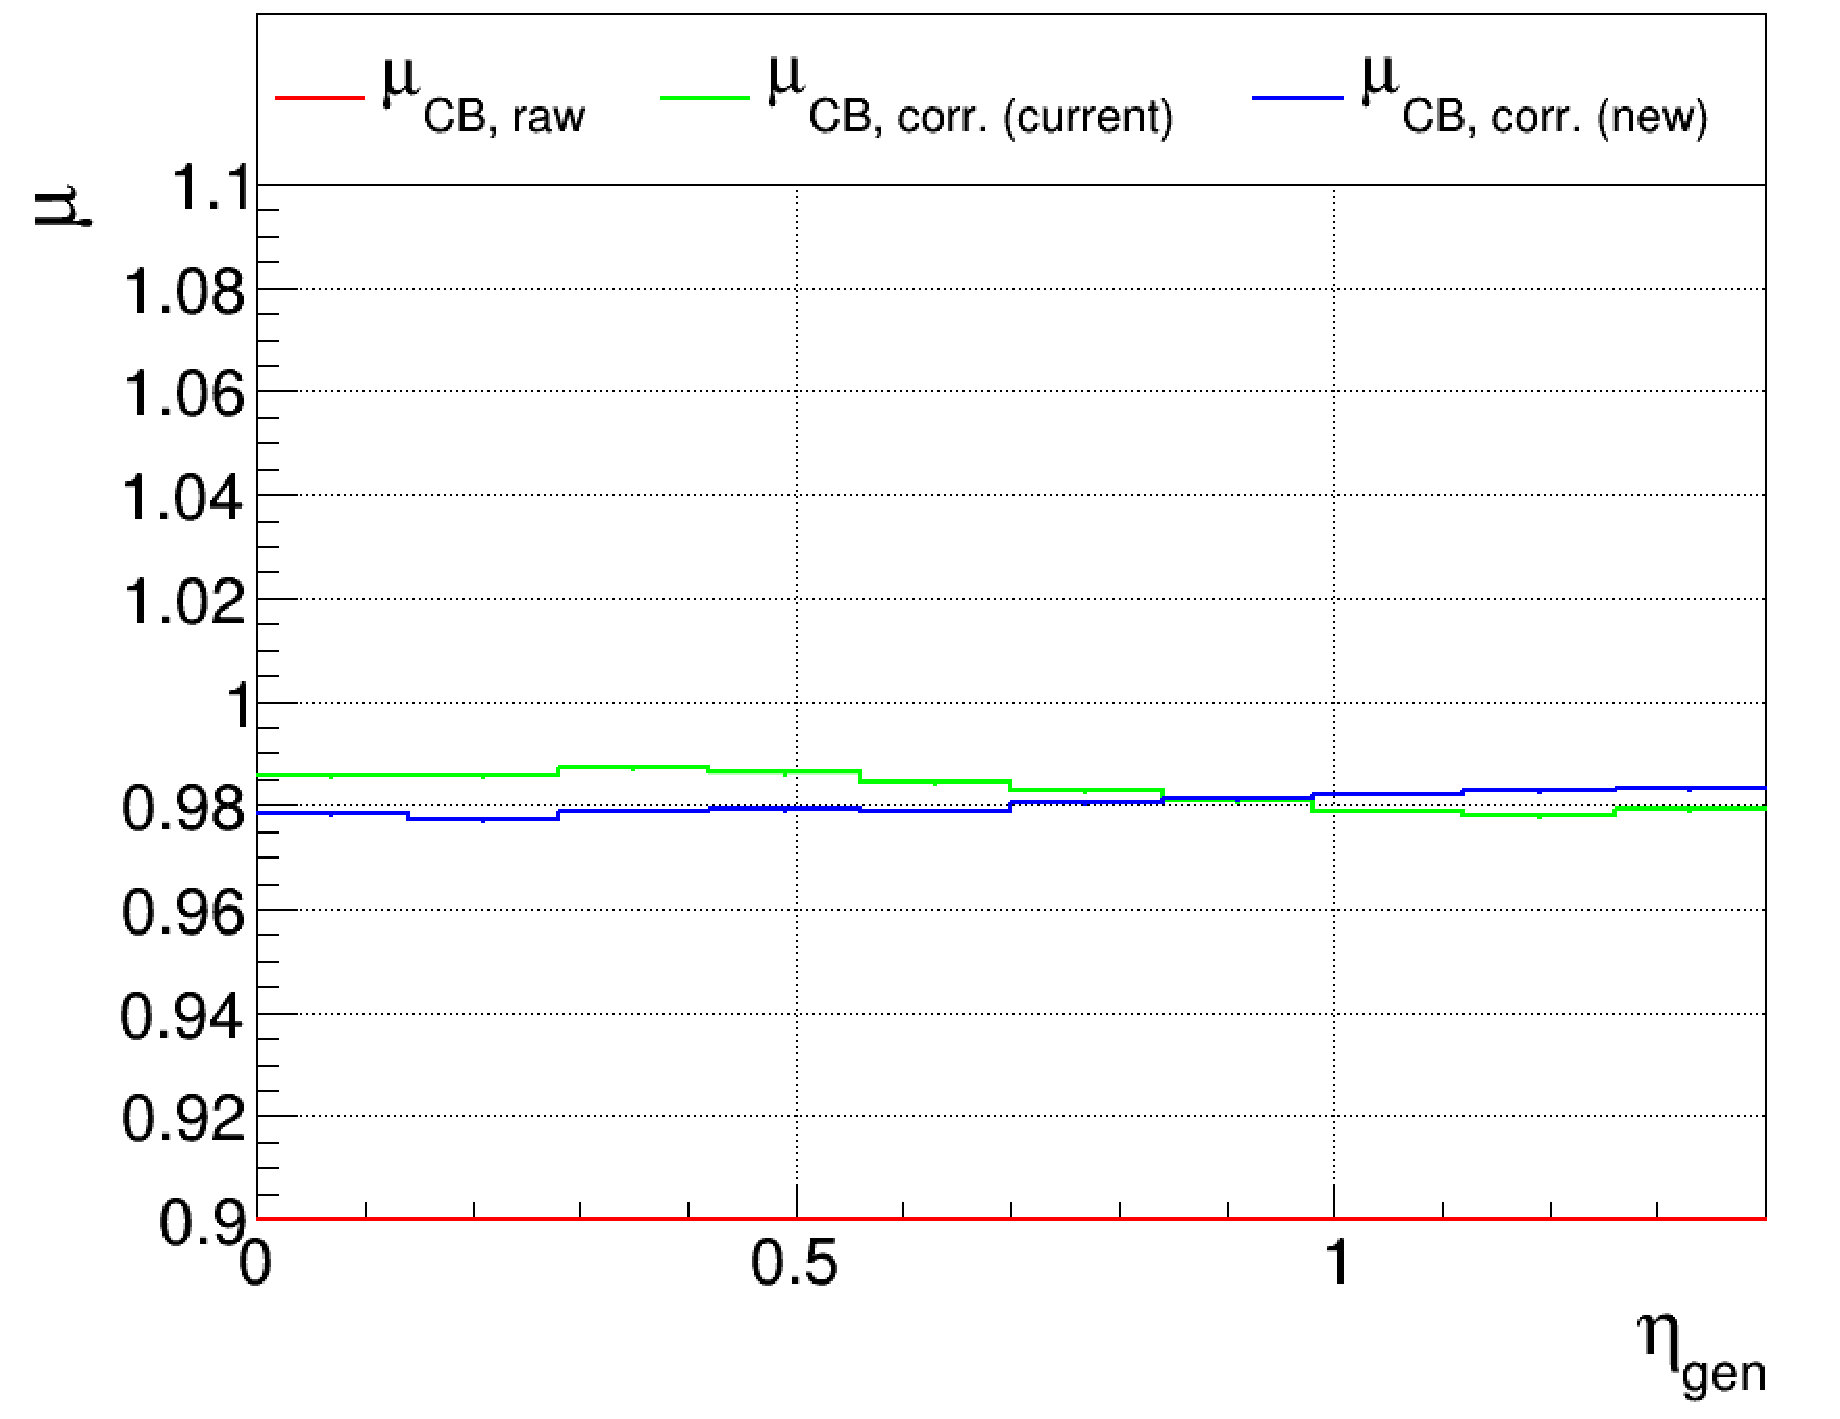
\includegraphics[width=0.495\textwidth]{./plots_pdf/ECAL_plots/plotsPU/EB/FULL/pdf/GENETA/EBFULL_GENETA_0005_0020_MuOverBins.pdf}
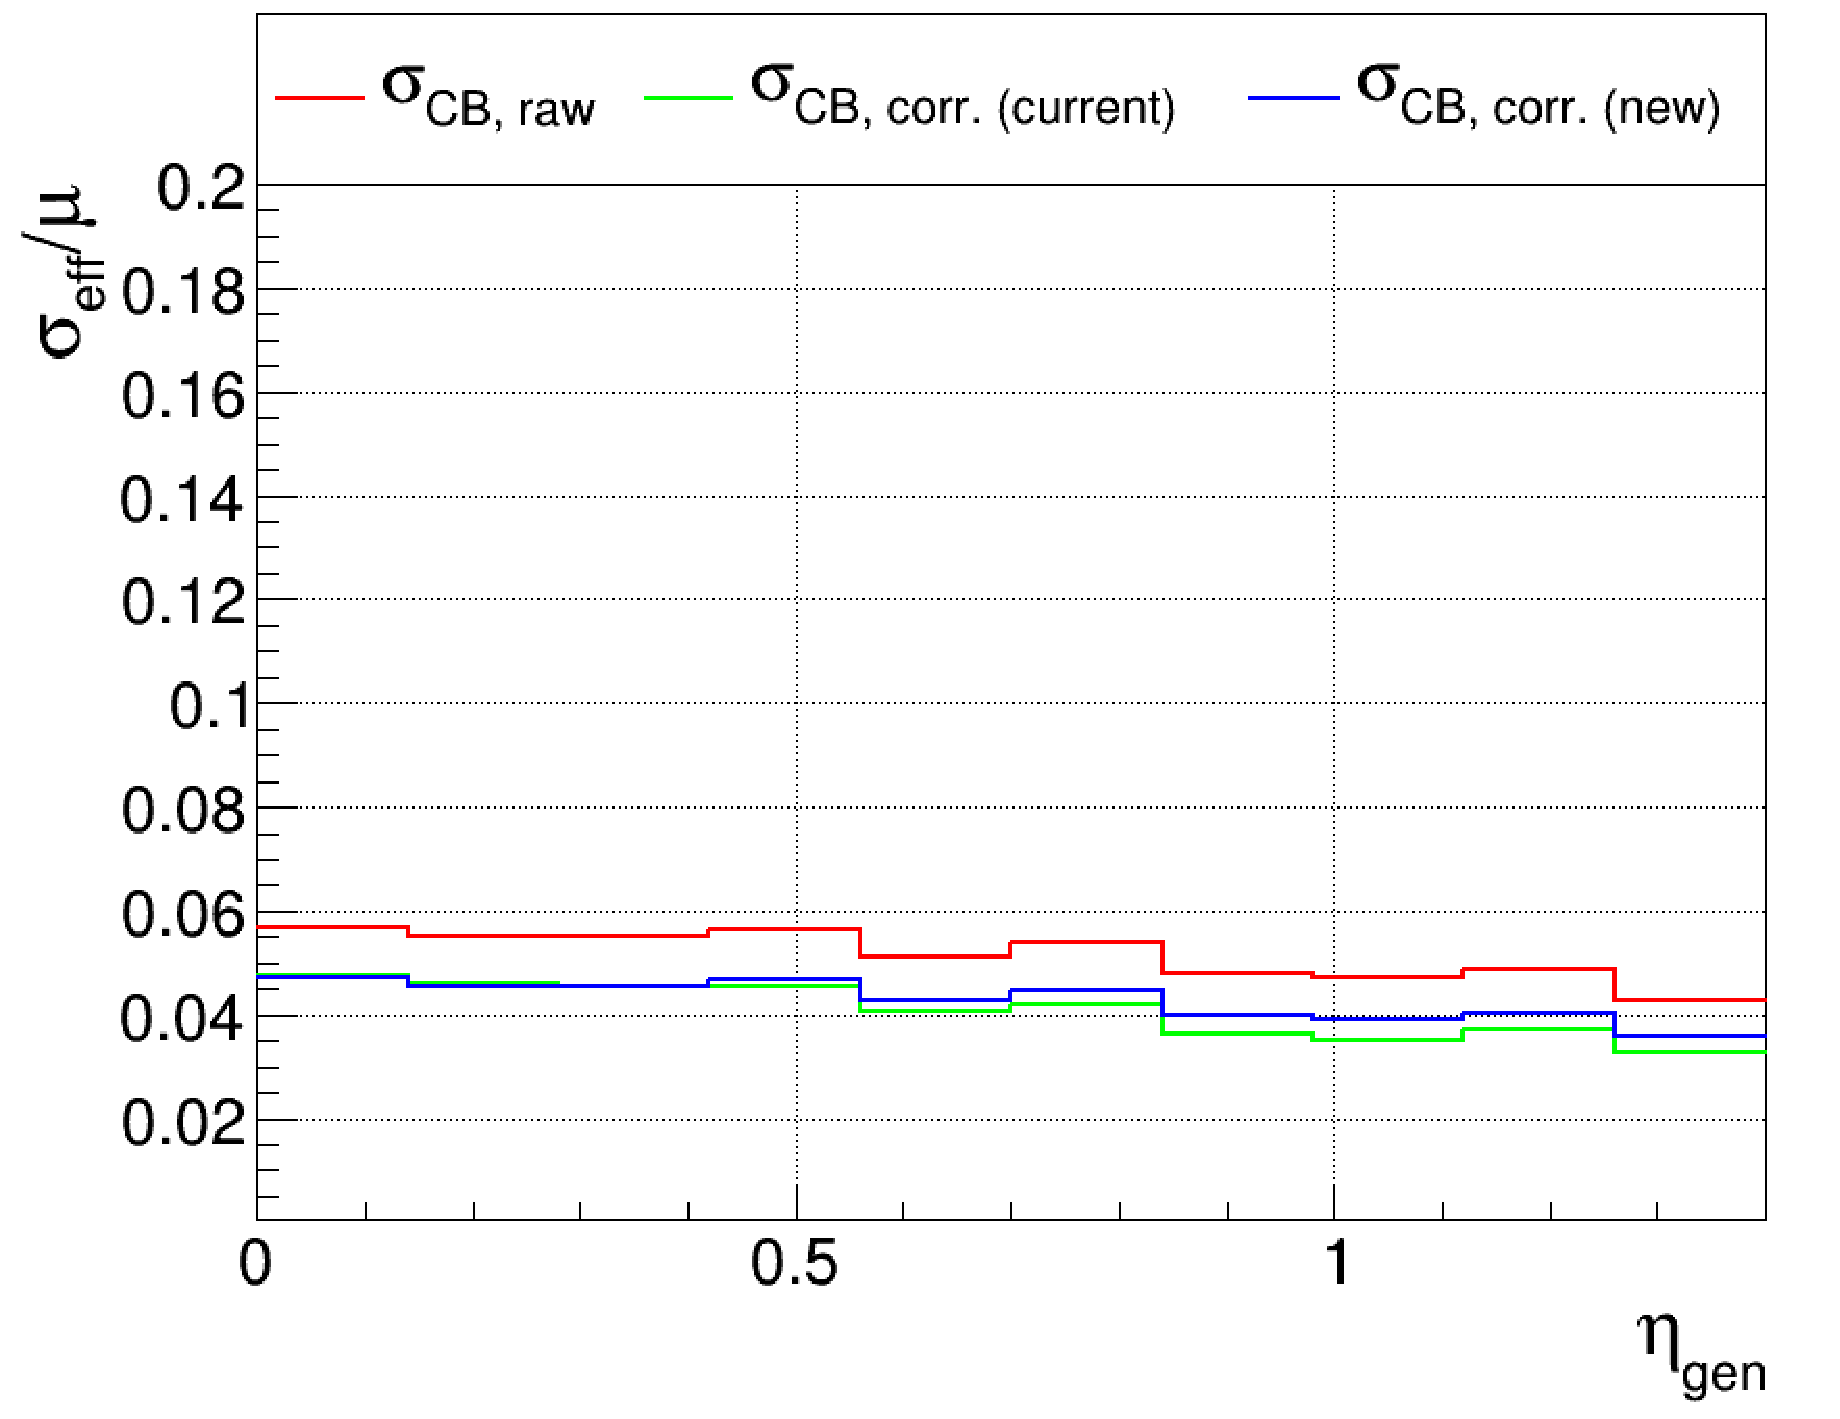
\includegraphics[width=0.495\textwidth]{./plots_pdf/ECAL_plots/plotsPU/EB/FULL/pdf/GENETA/EBFULL_GENETA_0005_0020_EffSigmaOverBins.pdf}

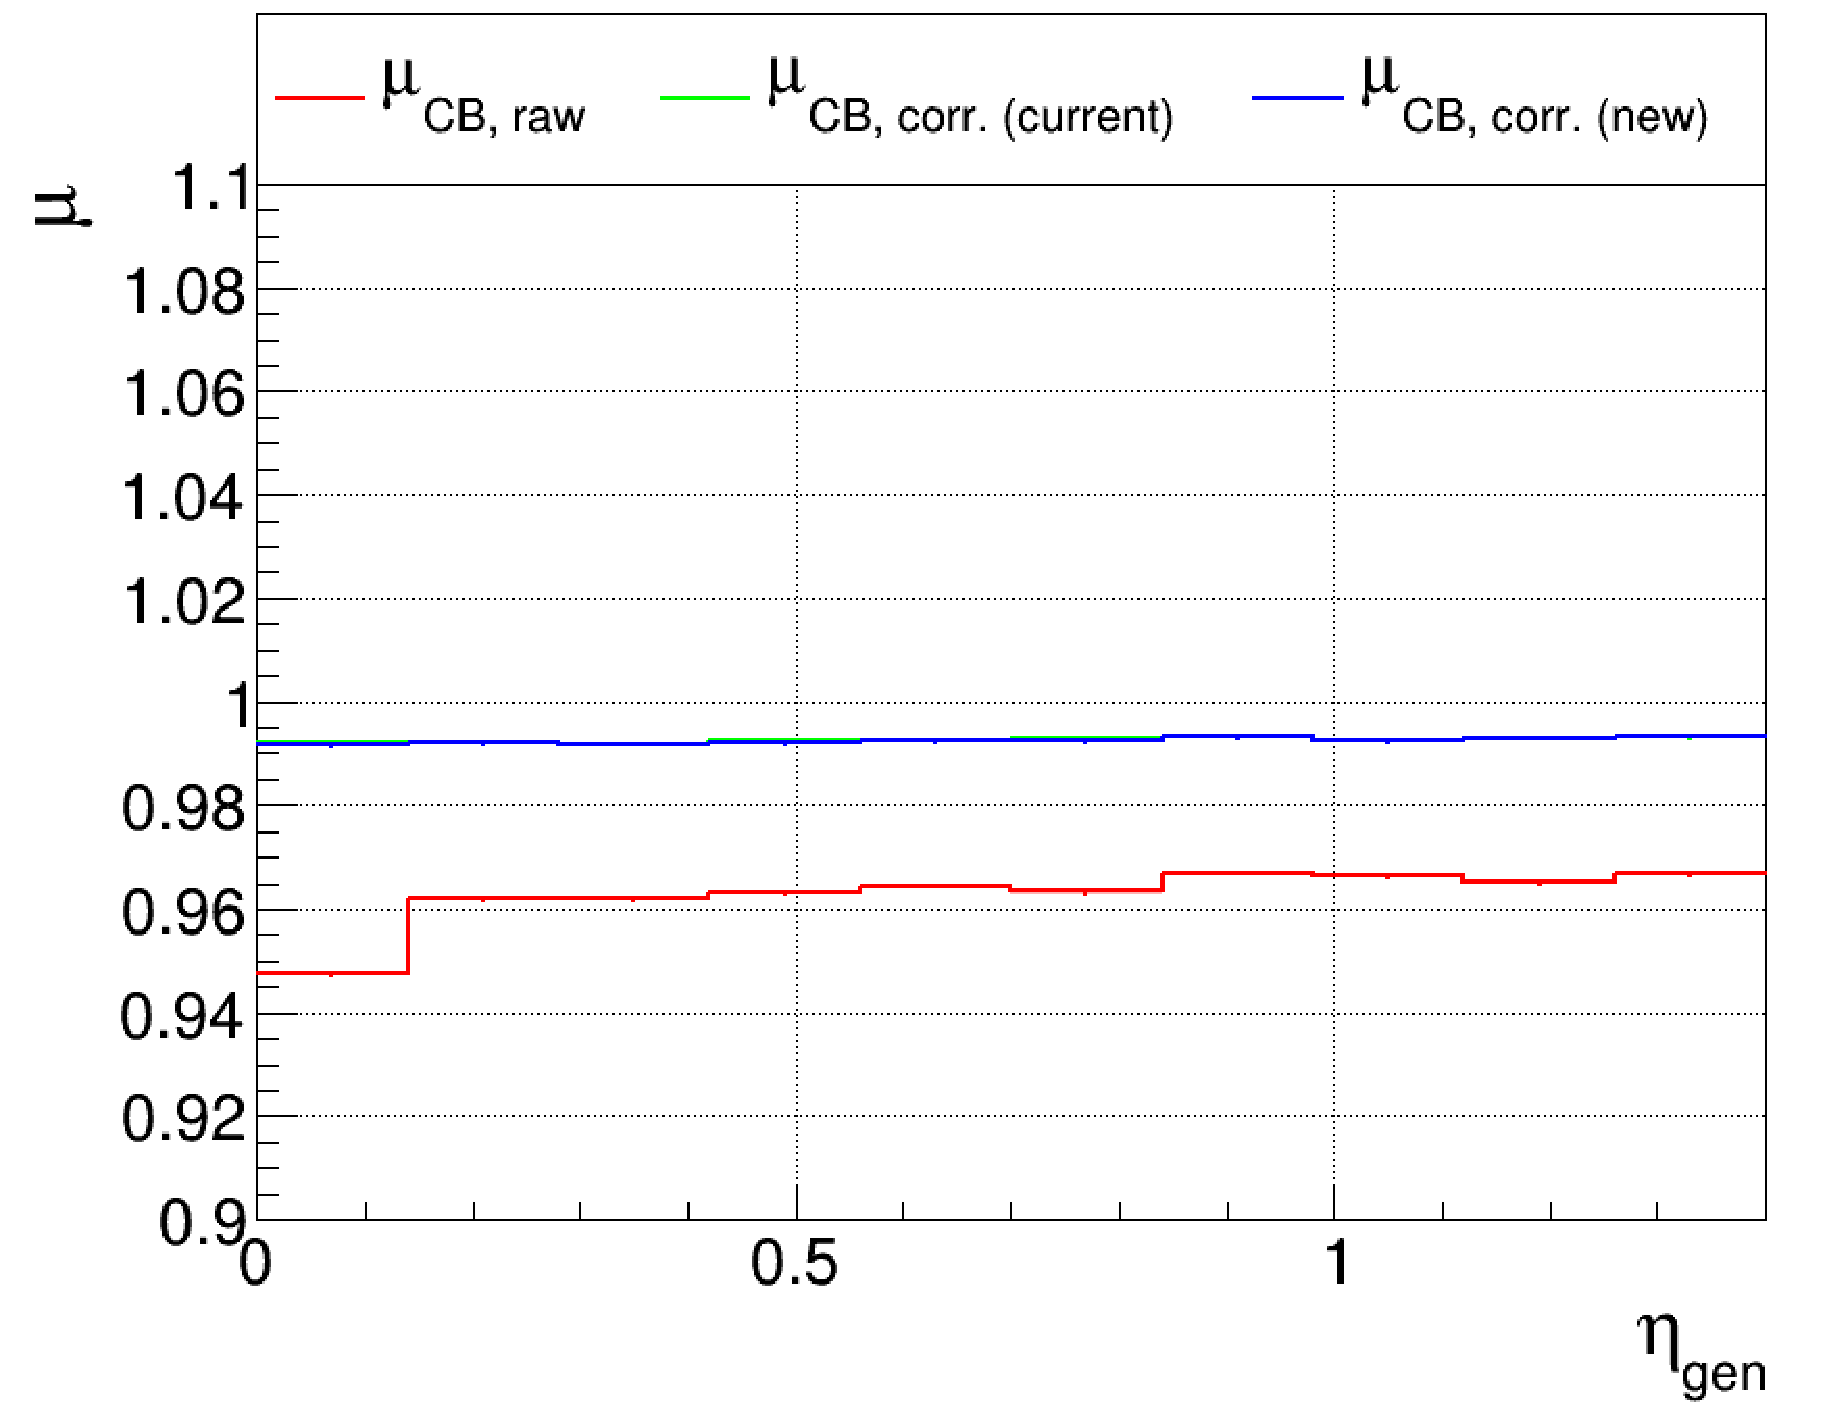
\includegraphics[width=0.495\textwidth]{./plots_pdf/ECAL_plots/plotsPU/EB/FULL/pdf/GENETA/EBFULL_GENETA_0020_0100_MuOverBins.pdf}
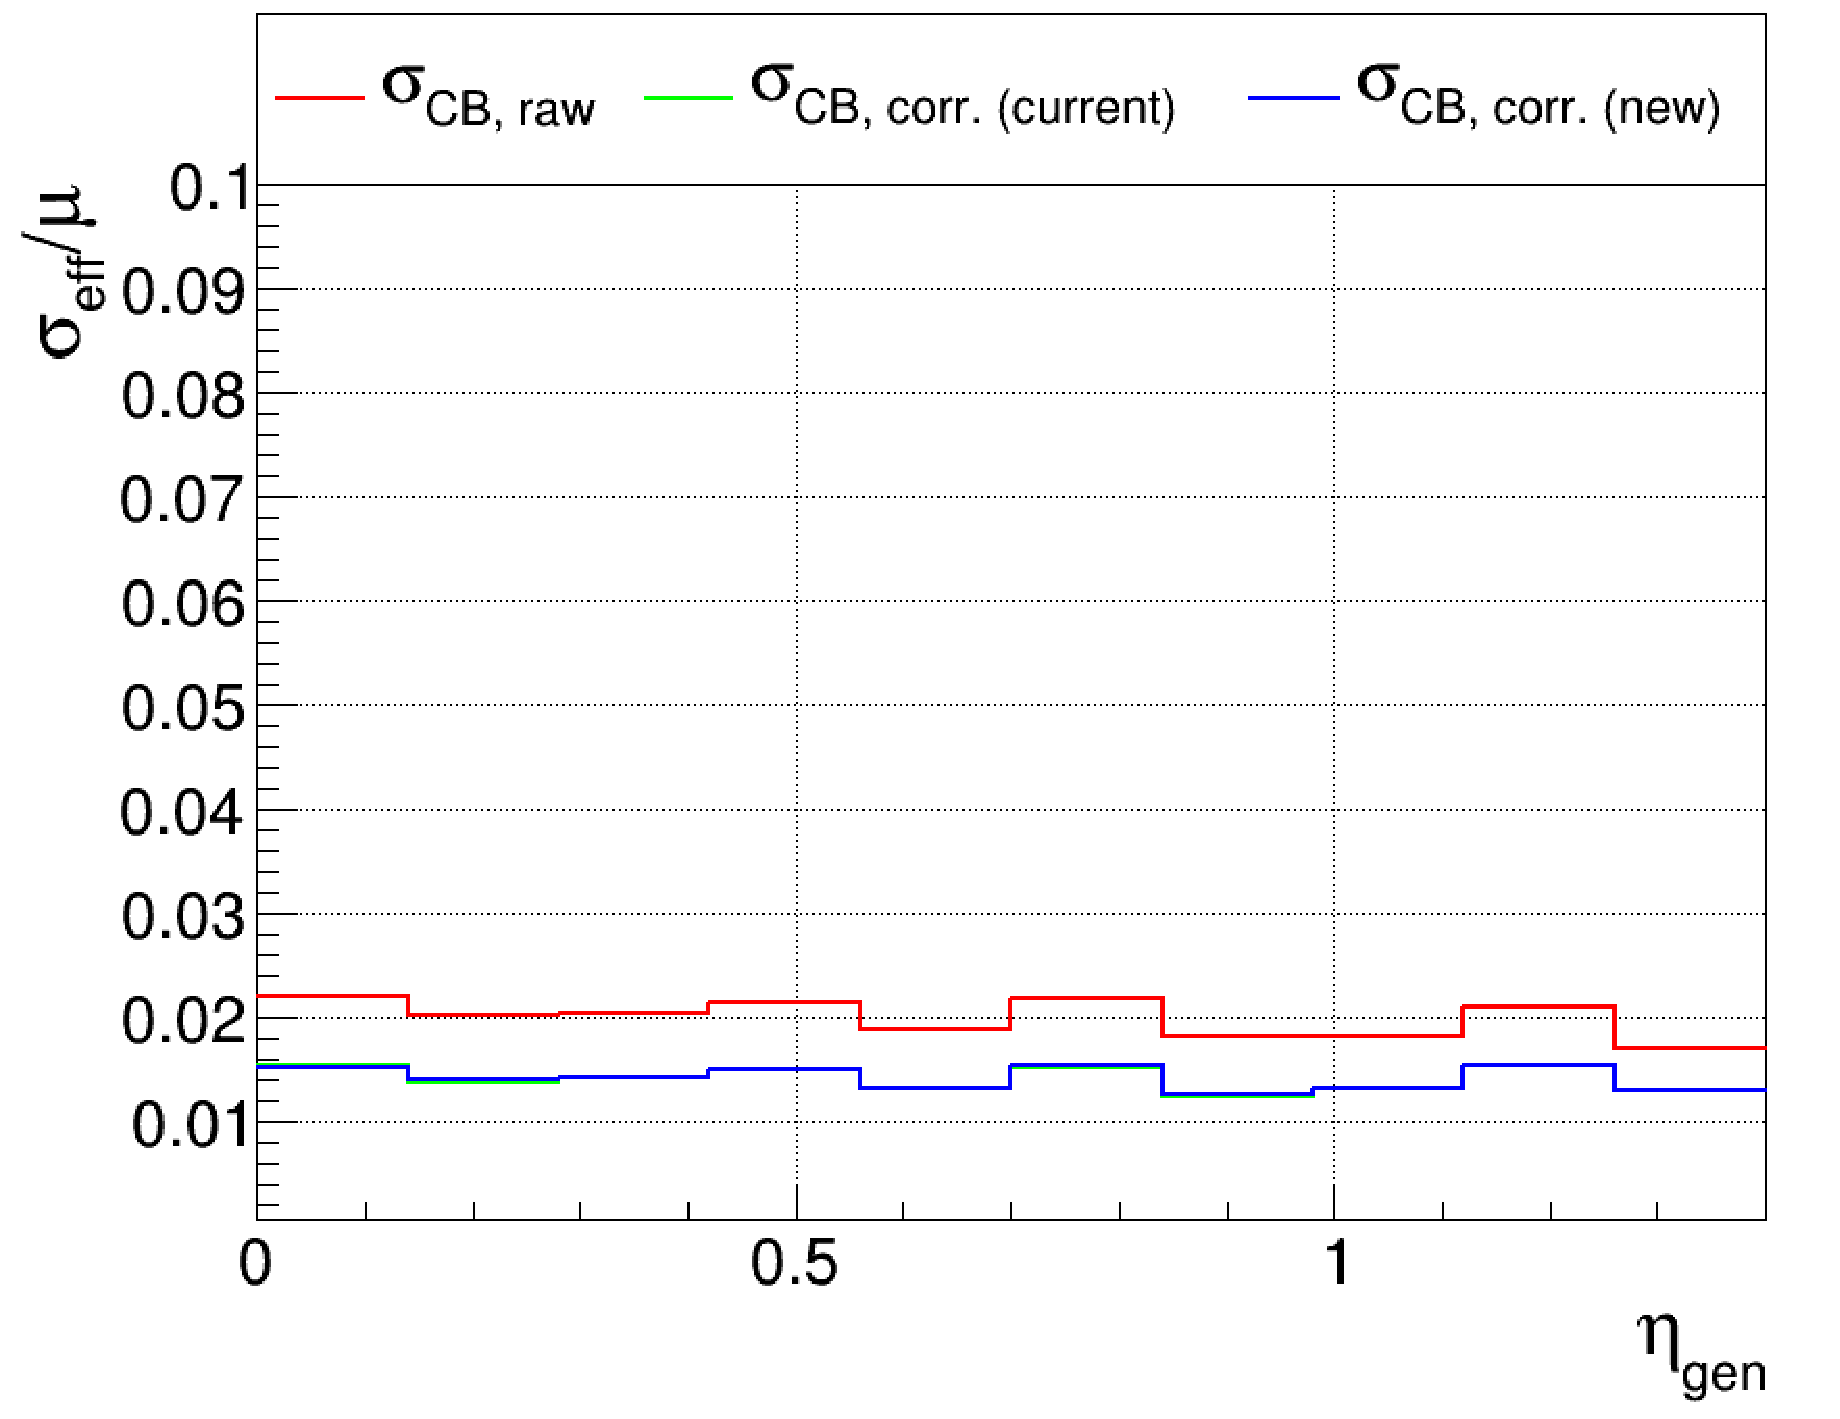
\includegraphics[width=0.495\textwidth]{./plots_pdf/ECAL_plots/plotsPU/EB/FULL/pdf/GENETA/EBFULL_GENETA_0020_0100_EffSigmaOverBins.pdf}

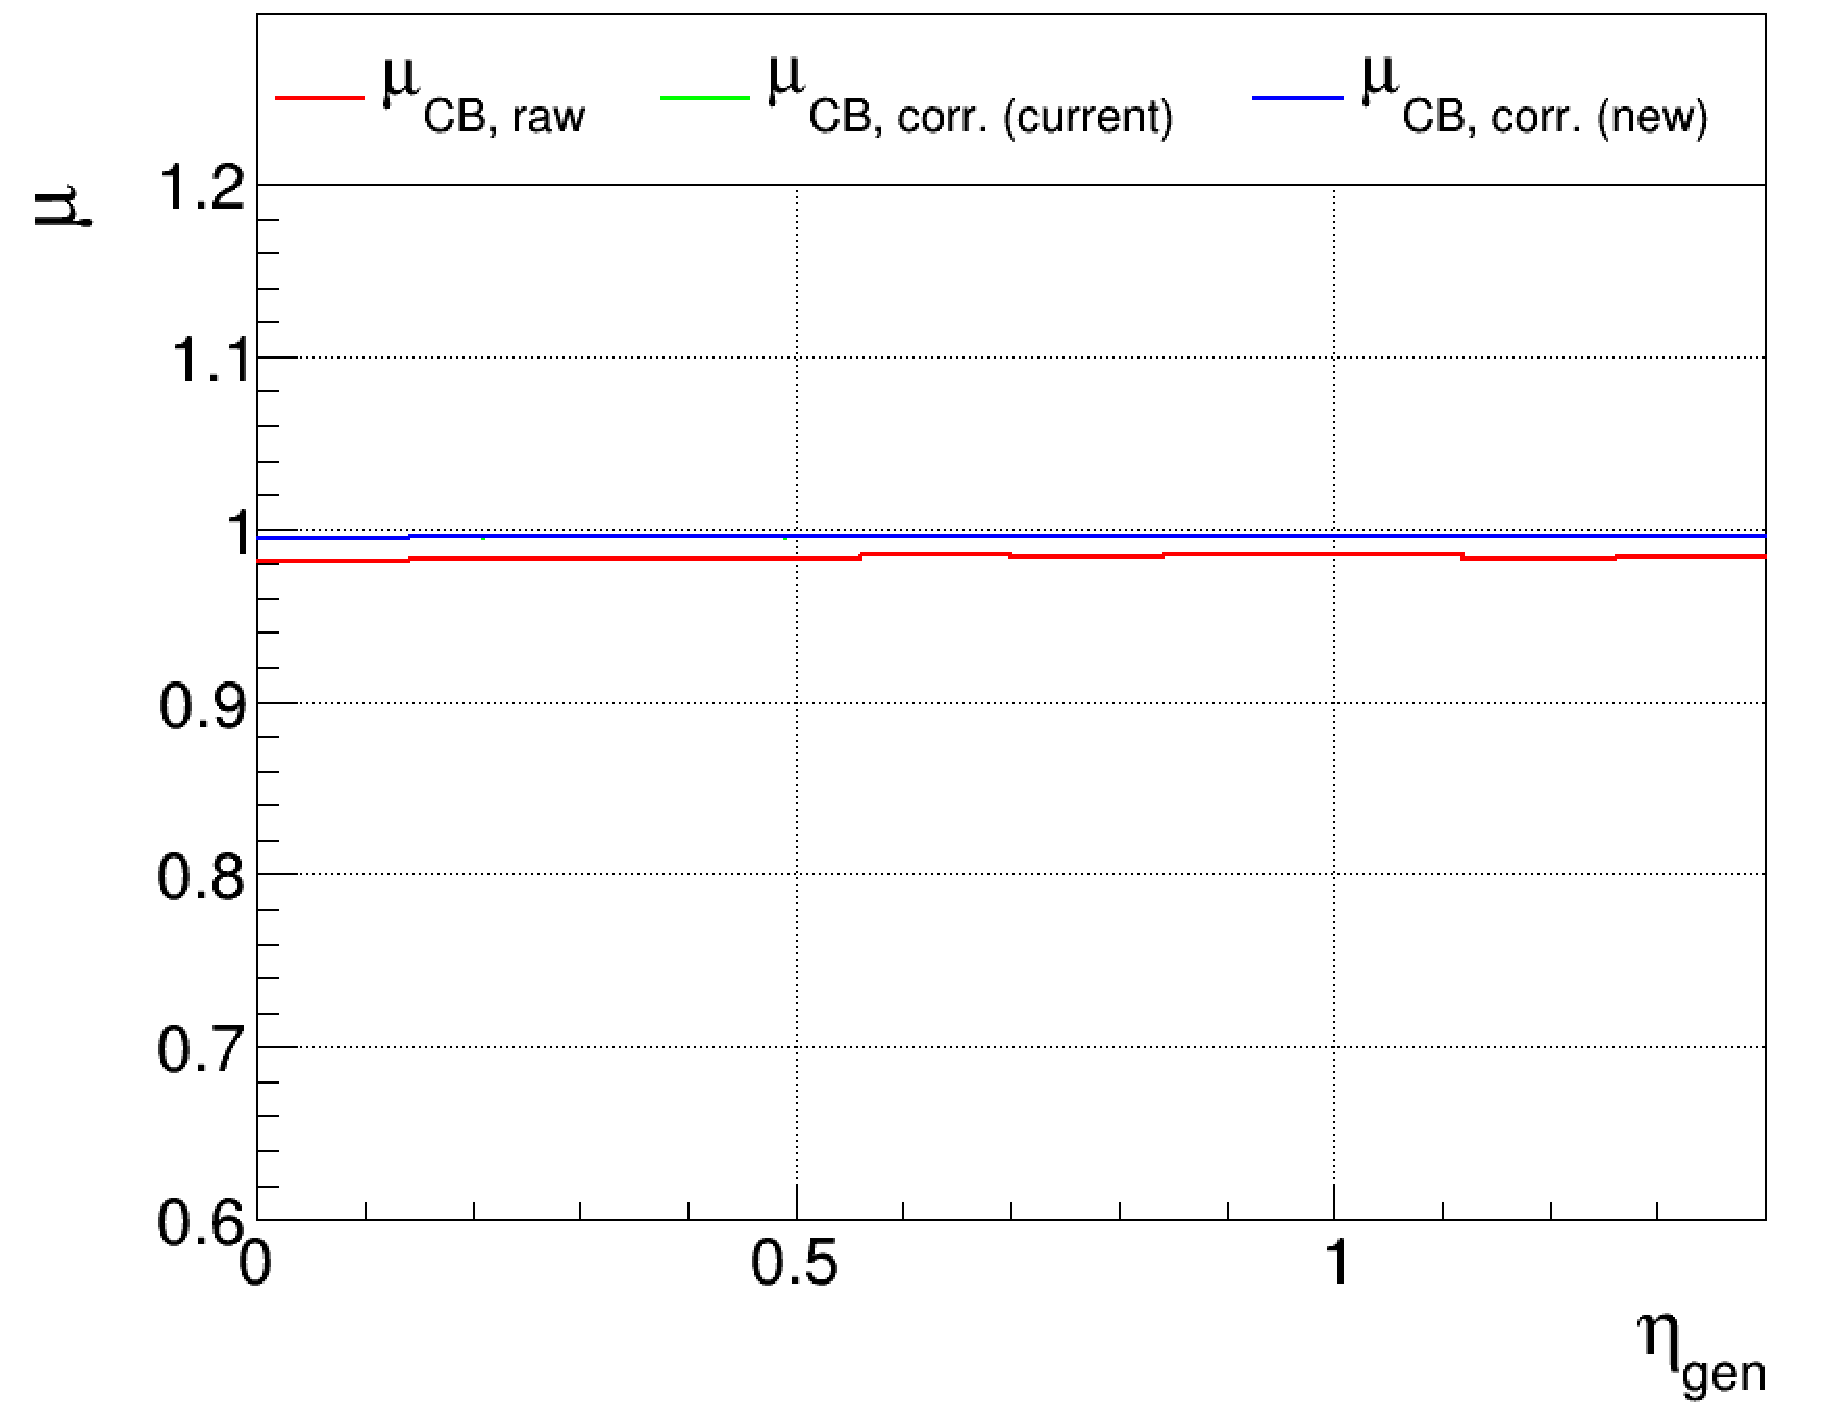
\includegraphics[width=0.495\textwidth]{./plots_pdf/ECAL_plots/plotsPU/EB/FULL/pdf/GENETA/EBFULL_GENETA_0100_0300_MuOverBins.pdf}
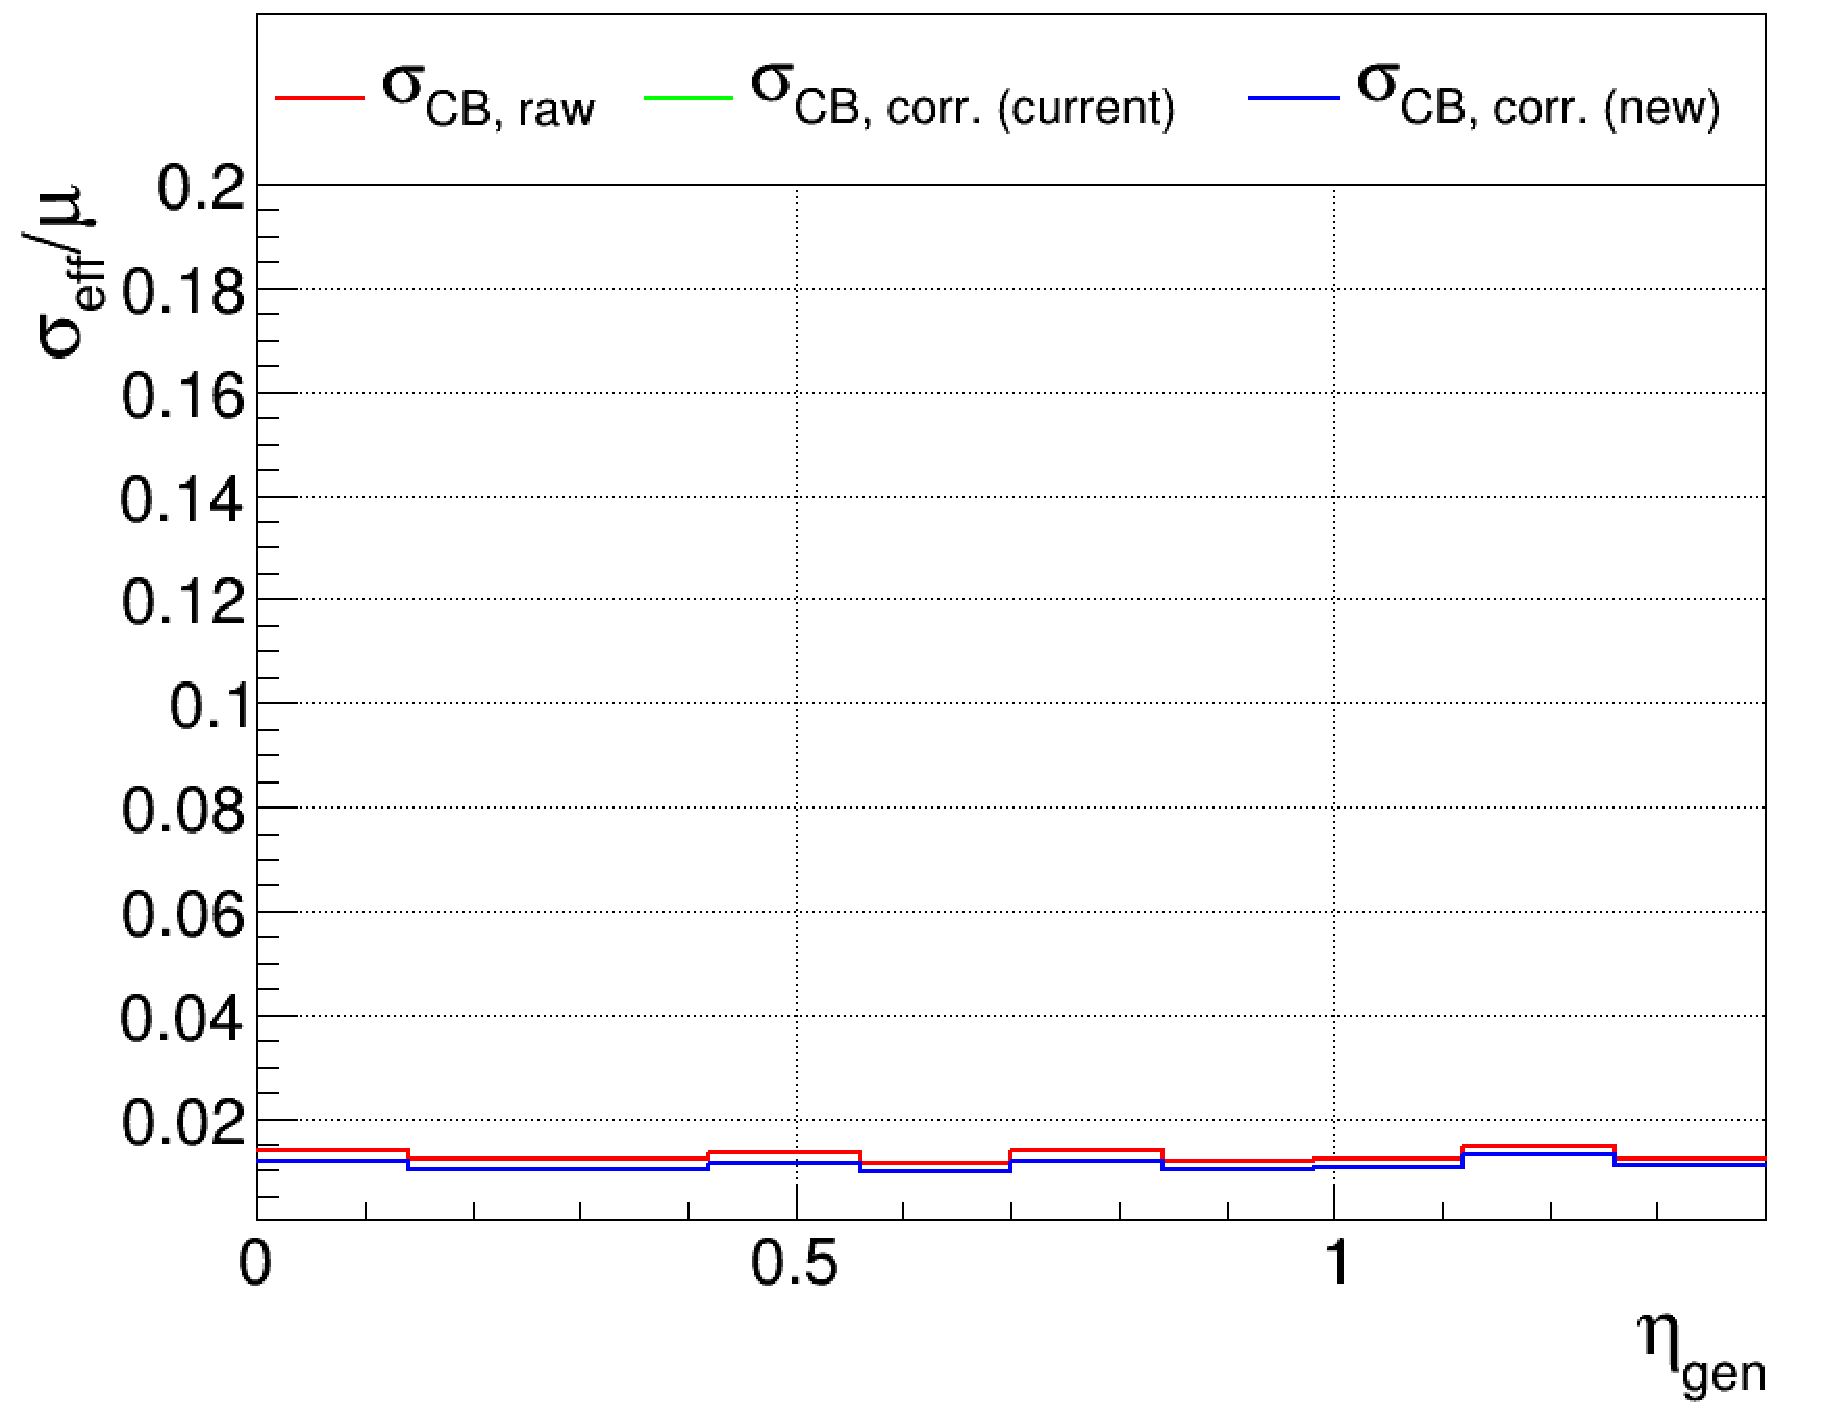
\includegraphics[width=0.495\textwidth]{./plots_pdf/ECAL_plots/plotsPU/EB/FULL/pdf/GENETA/EBFULL_GENETA_0100_0300_EffSigmaOverBins.pdf}

\caption [Energy response of PF ECAL cluster vs $\eta$ for PU EB Full readout senario]{PU EB Full Readout (top) low $\eta$, (middle) mid $\eta$, (bottom) high $\eta$}
\label{fig:PU_EBFULL_eta}
\end{figure}








